
%!TEX option = --shell-escape

\documentclass[9pt, xcolor={svgnames, x11names},professionalfonts]{beamer}


\usepackage{xcolor}
\usepackage{cancel}
\usepackage{bm}
\usepackage{graphicx}
\usepackage{hyperref}
\usepackage{adjustbox}
\hypersetup{colorlinks, allcolors=.,urlcolor=structure}
\usepackage{booktabs}  % for top and bottom spacing in table cells, \addlinespace
\usepackage[x11names, svgnames]{xcolor} % for colors in handouts, auto loaded in Beamer?
\usepackage{tikz}
\usetikzlibrary{arrows.meta, math, calc, shadows,bending}
\usetikzlibrary{decorations.markings, decorations.fractals, decorations.text} % for chain, etc.
\usetikzlibrary{intersections}
\usepackage{pgfmath}
\usepackage{ifthen}
\usepgfmodule{oo}
\usetikzlibrary{shadings}
% \usetikzlibrary{decorations.shapes}
\usepackage[many]{tcolorbox}
\tcbuselibrary{skins} % for image boxes
\usepackage[absolute,overlay,showboxes]{textpos}
% \usepackage{textpos}
% \textblockorigin{0.0cm}{0.0cm}  %start all at upper left corner
\TPshowboxesfalse

\newcommand\lb{\linebreak}
\newcommand\Ra{\Rightarrow}
\newcommand\cd{\!\cdot\!}
\newcommand\x{\!\times\!}
\newcommand\pars{\par\smallskip}
\newcommand\parm{\par\medskip}
\newcommand\parb{\par\bigskip}
\renewcommand{\deg}{^\circ}

% counter for resuming enumerated list numbers
\newcounter{resumeenumi}
\newcommand{\suspend}{\setcounter{resumeenumi}{\theenumi}}
\newcommand{\resume}{\setcounter{enumi}{\theresumeenumi}}



% https://tex.stackexchange.com/questions/33703/extract-x-y-coordinate-of-an-arbitrary-point-in-tikz
\makeatletter
\providecommand{\gettikzxy}[3]{%
	\tikz@scan@one@point\pgfutil@firstofone#1\relax
	\edef#2{\the\pgf@x}%
	\edef#3{\the\pgf@y}%
}
\makeatother

\makeatletter
\newcommand{\verbatimfont}[1]{\def\verbatim@font{#1}}%
\makeatother

%%%%%%%%%%%%%%%%%%%%%%%%%%%%%%%%%%%%%%%%%%%%%%%%%%%%%%%%%%%%%%%%%%%%%%%%%%%%%%%%


% \newcommand{\tb}[4][0.8]{
% 	\begin{textblock*}{#1}(#2, #3)
% 		\raggedright
% 		#4
% 	\end{textblock*}
% }

% \def\tb

\newtcolorbox{statsbox}[2][] { 
  colback=white,
  colbacktitle=structure,
  colframe=structure,
  coltitle=white,  
  top=0.25cm,
	bottom=0.125cm,
	left=0mm,
	right=0mm,
  % fonttitle=\itshape\rmfamily,
  halign=flush left, 
  enhanced,
  drop fuzzy shadow,
  attach boxed title to top left={xshift=3.5mm, yshift=-2mm},
  title={#2}, #1}
\newtcolorbox{redbox}{colback=white, colframe=structure, enhanced, drop fuzzy shadow}
\newtcolorbox{titledbox}[1]{colback=white,colframe=structure,title={#1}}
\newtcbox{\tcb}[1][]{colback=white,boxsep=0pt,top=0.5cm,bottom=0.5cm,left=0.5cm,
		right=0.5cm, colframe=structure,  enhanced, drop fuzzy shadow, #1}
\newtcbox{\tcbfig}[1][1]{colback=white,boxsep=0pt,top=0.5cm,bottom=0.5cm,left=0.5cm,
		right=0.5cm, colframe=structure,  enhanced, drop fuzzy shadow, #1}
% tcb title
\newtcbox{\tcbt}[2][]{colback=white,boxsep=0pt,top=5pt,bottom=5pt,left=5pt,
		right=5pt, colframe=structure, enhanced, drop fuzzy shadow,  title={#2}, #1}
% tcb left title
\newtcbox{\tcbtl}[2][]{ colback=white,
  colbacktitle=structure,
  colframe=structure,
  coltitle=white,  
  top=0.25cm,
	bottom=0.125cm,
	left=0mm,
	right=0mm,
  % fonttitle=\bfseries,
  halign=flush left, 
  enhanced,
  drop fuzzy shadow,
  attach boxed title to top left={xshift=3.5mm, yshift=-2mm}, 
	title={#2}, #1}

\newtcbtheorem{myexam}{Example}%
{
	enhanced,
	colback=white,
	colframe=structure,
	% fonttitle=\bfseries,
	fonttitle=\itshape\rmfamily,
	drop fuzzy shadow,
	%description font=\mdseries\itshape,
	attach boxed title to top left={yshift=-2mm, xshift=5mm},
	colbacktitle=structure
	}{exam}% then \pageref{exer:theoexample} references the theo

% \newcommand{\myexample}[2][red]{
% 	% \tcb\tcbset{theostyle/.style={colframe=red,colbacktitle=yellow}}
% 	\begin{myexam}{}{}
% 		#2
% 	\end{myexam}
% 	% \tcbset{colframe=structure,colbacktitle=structure}
% }

\newtcbtheorem{myexer}{Exercise}%
{
	enhanced,
	colback=white,
	colframe=structure,
	% fonttitle=\bfseries,
	drop fuzzy shadow,
	fonttitle=\itshape\rmfamily,
	% description font=\mdseries\itshape,
	attach boxed title to top left={yshift=-2mm, xshift=5mm},
	colbacktitle=structure
	}{exer}



\newcommand{\mini}[2][0.8]{
	\begin{minipage}[c]{#1\columnwidth}
		\raggedright
		#2
	\end{minipage}
}
\newcommand{\minit}[2][0.8]{
	\begin{minipage}[t]{#1\columnwidth}
		% \raggedright
		#2
	\end{minipage}
}

% centered minipage with text \raggedright
%\cmini[width]{content}
\newcommand{\cmini}[2][0.8]{
	\begin{center}
		\begin{minipage}{#1\columnwidth}
			\raggedright
			#2
		\end{minipage}
	\end{center}
}

\newcommand{\fig}[2][1]{% scaled graphic
	\includegraphics[scale=#1]{#2}
}

% centred framed box black border
%\cbox[width]{content}
\newcommand{\cbox}[2][1]{% framed centered color box
	\setlength\fboxsep{5mm}
	\setlength\fboxrule{.2 mm}
	\begin{center}
		\fcolorbox{black}{white}{
			\vspace{-0.5cm}
			\begin{minipage}{#1\columnwidth}
				\raggedright
				#2
			\end{minipage}
		}
	\end{center}
	\setlength\fboxsep{0cm}
}

\newcommand{\ccbox}[4][1]{% framed centered color box
	\setlength\fboxsep{5mm}
	\setlength\fboxrule{.2 mm}
	\begin{center}
		\fcolorbox{#2}{#3}{
			% \vspace{-0.5cm}
			\begin{minipage}{#1\columnwidth}
				\vspace{-0.25cm}
				\raggedright				
				#4
				\vspace{-0.325cm}
			\end{minipage}
		}
	\end{center}
	\setlength\fboxsep{0cm}
}

\newcommand{\cfig}[2][1]{% centred, scaled graphic
	\begin{center}
		% \fcolorbox{structure}{white}{
		\tcbincludegraphics{
			\includegraphics[scale=#1]{#2}
		}
	\end{center}
}

% figure with tight border for photos
% \cfigb[saitMaroon]{borderwidth with unit}{scale}{image}
\newcommand{\stcsfig}[2][1]{
	% \usepackage{adjustbox}
	% \setlength{\fboxrule}{1pt}
	\begin{center}
		\tcbincludegraphics[width=#1\textwidth, boxrule=2pt, top=-3pt, right=-3pt, left=-3pt, bottom=-3pt,colframe=structure, sharp corners, enhanced, drop fuzzy shadow]{#2}
	\end{center}
}






 \definecolor{saitPurple}{RGB}{112,40,119}
 \definecolor{statsMaroon}{rgb}{0.55, 0, 0}
 \definecolor{saitMaroon}{rgb}{0.55, 0, 0}
 \definecolor{saitRed}{RGB}{224,38,37}
 \definecolor{saitBlue}{rgb}{0, 0.59, 0.85}
 \definecolor{statsDeepBlue}{RGB}{0, 99, 167}
 \definecolor{saitDeepBlue}{RGB}{0, 99, 167}
 \definecolor{LightGrey}{RGB}{200,200,200}
%  \definecolor{boxBG}{RGB}{236, 227, 227}
%  \definecolor{boxBG}{RGB}{242, 233, 223}
% !TEX root = ../Beamer/statikz/statikz.tex

% \Channel[rotate=0]{coordinate}{draw}{fill}{scale}{lineWidth}
\newcommand{\Channel}[6][0]{
	\def\rotate{#1};
	\def\mid{#2}
	\def\lfill{#3}
	\def\lstroke{#4}
	\def\scale{#5};
	\def\lineWidth{#6};

	\begin{scope}[rounded corners=1pt, scale=\scale, rotate=\rotate]
		\filldraw[draw=\lstroke, fill=\lfill, line width=\lineWidth pt] ($(\mid) + (0,-3) $) -- ++(1.7,0) arc(0:85:0.25) -- ($ (\mid)+(0.4,-2.6) $) -- ($ (\mid)+(0.4,2.6) $) -- +(8.13:1.097)arc(-81.87:0:0.25) -- ($ (\mid)+(0,3) $)  -- cycle;
	\end{scope}
}

\newcommand{\Couple}[5][1]{
	\def\positive{#1};
	\def\lpin{#2}	
	\def\ldraw{#3}
	\def\diam{#4}
	\def\lwidth{#5}
	
	\begin{scope}[line cap = round]
		\ifthenelse{\equal{\positive}{1}}
			{
				\draw[line width=\lwidth mm, \ldraw, -{Latex[length=\lwidth*12, bend]}] ($ (\lpin)+(-150:\diam) $) arc (-150:165:\diam);
				% \draw[-latex, \ldraw, line width=\lwidth mm] ($ (\lpin)+(150:\diam) $) --+ (240:\lwidth/5);
			}
			{
				\draw[line width=\lwidth mm, \ldraw, -{Latex[length=\lwidth*12, bend]}] ($ (\lpin)+(150:\diam) $) arc (150:-165:\diam);
				% \draw[-latex, \ldraw, line width=\lwidth mm] ($ (\lpin)+(-140:\diam) $) --+ (120:\lwidth/5 );
			}
		
	\end{scope}
}
\newcommand{\DL}[9][1]{
  \def\forcedown{#1} % defaults to 1, force is downward
  \def\tl{#2} % top left, a coordinate
  \def\tr{#3} % top right. a coordinate
  \def\b{#4} % anywhere along the baseline (before any rotation), a coordinate 
  \def\lfill{#5} % background fill color
  \def\stroke{#6} % drawing color
  \def\spaces{#7} % number of spaces between arrows 
  \def\llinewidth{#8}
  \def\tiplength{#9}

  \gettikzxy{(\tl)}{\tlx}{\tly}
	\gettikzxy{(\tr)}{\trx}{\try}
	\gettikzxy{(\b)}{\bx}{\by}
  \pgfmathparse{abs(\try-\by)} \let\rlength\pgfmathresult
  \pgfmathparse{abs(\tly-\by)} \let\llength\pgfmathresult

  \fill[\lfill] (\tlx, \tly)--(\trx, \try)--(\trx, \by)--(\tlx, \by);
  \draw[\stroke, line cap = round, line width = \llinewidth mm] (\tl)--(\tr);
  
  % no empty lines in \tikzmath!
  \tikzmath{
    % Calculate the width of the load, and the spacing between arrows
    % Also, calculate the difference in length between adjacent arrows.
    \dx = \trx - \tlx; % width of dist load
    \dx = \dx / \spaces; % space between arrows
    \dy = \try - \tly; % difference between two load values
    \dy = \dy / \spaces; % difference between arrow-line lengths
    %    
    if \forcedown == 1 then {       
			for \i in {0,...,\spaces} {	
        \starty = \tly+\i*\dy;
        \length = \starty-\by;
        % in \tikzmath, drawing commands are enclosed in { }; 
        {
          \begin{scope}          
            \clip (\tlx,\tly) -- (\trx, \try) -- (\trx,\by) --(\tlx,\by);
            \draw[\stroke, line width = \llinewidth mm, -{Latex[length=\tiplength]}](\tlx+\i*\dx, \starty pt)-- +(270: \length pt);
          \end{scope}
        };
			};
    } else {
      for \i in {0,...,\spaces} {	
        \starty = \tly+\i*\dy;
        \length = \starty-\by;			
				{
          \begin{scope}          
            \clip (\tlx,\tly) -- (\trx, \try) -- (\trx,\by) --(\tlx,\by);
            \draw[\stroke, line width = \llinewidth mm, {Latex[length=\tiplength]}-](\tlx+\i*\dx, \starty pt)-- +(270: \length pt);
          \end{scope}          
        };
			};      
    };
    if \forcedown == 1 then {
      if \rlength > \tiplength then {
        {\draw[\stroke, line width = \llinewidth mm, -{Latex[length=\tiplength]}] (\trx, \try)--(\trx, \by);};
      } else {
         {\draw[\stroke, line width = \llinewidth mm] (\trx, \try)--(\trx, \by);};
      };    
      if \llength > \tiplength then {
        {\draw[\stroke, line width = \llinewidth mm, -{Latex[length=\tiplength]}] (\tlx, \tly)--(\tlx, \by);};
      } else {
        {\draw[\stroke, line width = \llinewidth mm] (\tlx, \tly)--(\tlx, \by);};
      };
    } else {
      if \rlength > \tiplength then {
        {\draw[\stroke, line width = \llinewidth mm, {Latex[length=\tiplength]}-] (\trx, \try)--(\trx, \by);};
      } else {
        {\draw[\stroke, line width = \llinewidth mm] (\trx, \try)--(\trx, \by);};
      };    
      if \llength > \tiplength then {
        {\draw[\stroke, line width = \llinewidth mm, {Latex[length=\tiplength]}-] (\tlx, \tly)--(\tlx, \by);};
      } else {
        {\draw[\stroke, line width = \llinewidth mm] (\tlx, \tly)--(\tlx, \by);};
      };
    };    
  } % \end tikzmath environment
} % end of \DL definition
\input{../../includes/DLdown.tex}
% !TEX root = ../Beamer/02ForceVectors/02ForceVectors.tex


\newcommand{\EyeBolt}[6][0]{
	\def\lrotate{#1};
	\def\lpin{#2}
	\def\lfill{#3}
	\def\ldraw{#4}
	\def\lscale{#5}
	\def\lwidth{#6}
	%\def\h{1.5}
	\def\r{0.3}
	\begin{scope}[scale=\lscale, rotate=\lrotate]
		\filldraw[draw=\ldraw, fill=\lfill, line width=\lwidth pt] ($(\lpin) + (-0.7,-1.25)$) arc(180:90:.2) -- ++(0.05,0)arc(-90:0:0.2) -- ++(0.05,0.65)arc(225:-45:0.28284)-- ++(0.05,-.65)arc(180:270:.2)-- ++(0.05,0)arc(90:0:0.2) -- cycle;
		\fill[outer color=\lfill, inner color=black, line width = 0] (\lpin) circle (2.25mm);
		\filldraw[fill=white, draw=\ldraw, line width = \lwidth pt] (\lpin) circle (1.25mm);

		\begin{scope}[even odd rule]
			\fill[\lfill] (\lpin) circle (2.5mm)
			(\lpin) circle (2.125mm);
		\end{scope}

		\filldraw[rounded corners=\lscale pt, draw=\ldraw, fill=\lfill, line width=\lwidth pt] ($ (\lpin) - (1,1.5) $) rectangle +(2,0.25);
	\end{scope}
}

% !TEX root = ../../Beamer/statikz/statikz.tex


\newcommand{\EyeConnection}[6][0]{
	\def\lrotate{#1};
	\def\lpin{#2}
	\def\lfill{#3}
	\def\ldraw{#4}
	\def\lscale{#5}
	\def\lwidth{#6}
	\def\h{1}
	\def\r{0.3}
	\begin{scope}[scale=\lscale, rotate=\lrotate]
		\filldraw[draw=\ldraw, fill=\lfill, line width=\lwidth pt] ($(\lpin) + (0.201*\h+1.0353*\r ,-0.75*\h)$) -- ++(105: 0.77646*\h+0.26795*\r) arc (15:165:\r) -- ++(-105:0.77646*\h+0.26795*\r) -- cycle;

		\fill[outer color=\lfill, middle color=red, inner color=black, line width = \lwidth pt] (\lpin) circle (2.5mm);
		\filldraw[fill=white, draw=\ldraw, line width = \lwidth pt] (\lpin) circle (1.25mm);

		\filldraw[rounded corners=\lscale pt, draw=\ldraw, fill=\lfill, line width=\lwidth pt] ($ (\lpin) - (1,1) $) rectangle +(2,0.25);
	\end{scope}
}

%\Member{startpt}{endpt}{outer fill color}{inner fill color}{stroke}{height}{radius}{linewidth}
\providecommand{\Member}[8]{
  % name the points
  \coordinate(start) at (#1);
  \coordinate(end) at (#2);
  \edef\ofill{#3}%
  \edef\ifill{#4}%
  \edef\stroke{#5}%
  \edef\height{#6} % cm
  \edef\radius{#7} % cm
  \edef\linewidth{#8} % mm

  \coordinate(delta) at ($ (end)-(start) $);
  \gettikzxy{(delta)}{\dx}{\dy}
  \gettikzxy{(start)}{\sx}{\sy}
  \pgfmathparse{veclen(\dx, \dy)} \let\length\pgfmathresult

  \pgfmathparse{\dx==0}%
  % \ifnum low-level TeX for integers
  \ifnum\pgfmathresult=1 % \dx == 0
    \pgfmathsetmacro{\rot}{\dy > 0 ? 90 : -90}
  \else
    \pgfmathsetmacro{\rot}{\dx > 0 ? atan(\dy / \dx) : 180 + atan(\dy / \dx)}
  \fi

  
   
  \shadedraw[transform canvas = { rotate around = {\rot:(\sx,\sy)}}, line width = \linewidth, rounded corners = \radius mm, top color = \ofill, bottom color = \ofill, middle color = \ifill, draw = \stroke] ($ (start)+(-0.5*\height, 0.5*\height) $) -- ++(\height cm +\length pt, 0 ) -- ++(0, -\height) -- ++ (-\height cm -\length pt, 0) -- cycle;


  \shadedraw[ball color = \ofill!50!\ifill, draw = \stroke] (start) circle (\height/8);
  \shadedraw[ball color = \ofill!50!\ifill, draw = \stroke] (end) circle (\height/8);
  %  \pgfresetboundingbox

  
  


}

%\Member{startpt}{endpt}{outer fill color}{inner fill color}{stroke}{height}{radius}{linewidth}
\providecommand{\Mem}[8]{
  % name the points
  \coordinate(start) at (#1);
  \coordinate(end) at (#2);
  \edef\ofill{#3}%
  \edef\ifill{#4}%
  \edef\stroke{#5}%
  \edef\height{#6} % cm
  \edef\radius{#7} % cm
  \edef\linewidth{#8} % mm

  \coordinate(delta) at ($ (end)-(start) $);
  \gettikzxy{(delta)}{\dx}{\dy}
  \gettikzxy{(start)}{\sx}{\sy}
  \gettikzxy{(end)}{\ex}{\ey}
  \pgfmathparse{veclen(\dx, \dy)} \let\length\pgfmathresult

  \pgfmathparse{\dx==0}%
  % \ifnum low-level TeX for integers
  \ifnum\pgfmathresult=1 % \dx == 0
    \pgfmathsetmacro{\rot}{\dy > 0 ? 90 : -90}
  \else
    \pgfmathsetmacro{\rot}{\dx > 0 ? atan(\dy / \dx) : 180 + atan(\dy / \dx)}
  \fi
  \pgfmathparse{\dy==0}%
  % \ifnum\pgfmathresult=1 % \dx == 0
  %   \pgfmathsetmacro{\rot}{\dy > 0 ? 0 : 180}
  % \fi

  \pgfdeclareverticalshading{myshading}{\length pt}{
    color(0)=(\ofill); color(0.5*\length pt-0.5*\height cm)=(\ofill); color(0.5*\length pt)=(\ifill); color(0.5*\length pt+0.5*\height cm)=(\ofill); color(\length pt)=(\ofill)
  }

  
  \begin{scope}[shading=myshading] 
    \shadedraw[rotate around = {\rot:(\sx,\sy)}, line width = \linewidth mm, rounded corners = \radius cm, draw = \stroke, shading angle=\rot] ($ (\sx,\sy)+(-0.5*\height cm, 0.5*\height cm) $) -- ++(\height cm +\length pt, 0 ) -- ++(0, -\height cm) -- ++ (-\height cm -\length pt, 0) -- cycle;
    %  \node[below] at (\sx, \sy) {\length};
  \end{scope}

%  \pgfresetboundingbox
  \shadedraw[ball color = \ofill!50!\ifill, draw = \stroke] (start) circle (\height/8);
  \shadedraw[ball color = \ofill!50!\ifill, draw = \stroke] (end) circle (\height/8);
  

  % \node at (\ex,\ey+1cm){$\rot\deg$};
  


}

%\Member{startpt}{endpt}{outer fill color}{inner fill color}{stroke}{height}{radius}{linewidth}
\providecommand{\Meme}[8]{
  \coordinate(start) at (#1);
  \coordinate(end) at (#2);
  \edef\ofill{#3}%
  \edef\ifill{#4}%
  \edef\stroke{#5}%
  \edef\height{#6} % cm
  \edef\radius{#7} % cm, should be half \height or less
  \edef\linewidth{#8} % mm

  


  \coordinate(delta) at ($ (end)-(start) $);
  \gettikzxy{(delta)}{\dx}{\dy}
  \gettikzxy{(start)}{\sx}{\sy}
  \gettikzxy{(end)}{\ex}{\ey}
  \pgfmathparse{veclen(\dx, \dy)} \let\length\pgfmathresult
  \pgfmathparse{\height*28.435} \let\heightpt\pgfmathresult
  \pgfmathparse{\heightpt/\length} \let\ratio\pgfmathresult
  \pgfmathparse{1/\ratio} \let\inverse\pgfmathresult
  

  \pgfmathparse{\dx==0}%
  % \ifnum low-level TeX for integers
  \ifnum\pgfmathresult=1 % \dx == 0
    \pgfmathsetmacro{\rot}{\dy > 0 ? 90 : -90}
  \else
    \pgfmathsetmacro{\rot}{\dx > 0 ? atan(\dy / \dx) : 180 + atan(\dy / \dx)}
  \fi

  \pgfmathparse{round(mod(abs(\rot),90))} \let\tmp\pgfmathresult
  \pgfmathsetmacro{\rotmod}{\tmp>45?90-\tmp:\tmp}
  \pgfmathparse{(0.007*\rotmod-0.315)/45+1.017} \let\rotfudge\pgfmathresult

  % \pgfmathparse{mod(abs(\rot),90)} \let\moded\pgfmathresult
  % \ifthenelse{\moded>45}{
  %   \pgfmathparse{90-\moded} \let\rotmod\pgfmathresult    
  % }{
  %   \pgfmathparse{div(\moded,1)} \let\rotmod\pgfmathresult   
  % }


  
  \pgfmathparse{1+3.62/(1+(\inverse/0.714)^1.69)} \let\fudge\pgfmathresult
  \pgfmathparse{50*(1-\ratio)*\fudge*\rotfudge} \let\colorstop\pgfmathresult
  \pgfmathparse{(100-\colorstop)} \let\colorstoptwo\pgfmathresult

  \pgfdeclareverticalshading{myshade}{100bp}{%
					color(0bp)=(\ofill);
					% color(\colorstop bp)=(\ofill);
					color(\colorstop bp)=(\ofill);
					color(50 bp)=(\ifill);
					color(\colorstoptwo bp)=(\ofill);
					color(100bp)=(\ofill)}

  % \tikzset{shading=myshade}

  \begin{scope}[rotate around = {\rot:(start)}, rounded corners = \radius cm, shading angle=\rot]
    \begin{scope} 
      \path[clip]($ (start)+(-0.5*\height, 0.5*\height cm) $) rectangle +(\length pt+\height cm, -\height);
      \shade[shading=myshade] ($ (start)+(-0.5*\height, 0.5*\length pt) $) rectangle +(\length pt+\height cm, -\length pt);
    \end{scope}
  \draw[line width=\linewidth, \stroke] ($ (start)+(-0.5*\height, 0.5*\height cm) $) rectangle +(\length pt+\height cm, -\height);

  % \shadedraw[top color=\ofill, bottom color=\ofill, middle color=\ifill, rotate around = {\rot:(start)}, draw=\stroke, rounded corners = \radius cm, , shading angle=\rot] ($ (start)+(-0.5*\height cm, 0.5*\length pt) $) rectangle +(\length pt+\height cm, -\length pt);
  \end{scope}

  % \pgfresetboundingbox


  % \node[orange] at (0,-1) {rot: \rot};  
  % \node[orange] at (0,-1.5) {rotmod: \rotmod};  
  % \node[orange] at (0,-2) {rotfudge: \rotfudge};  
  % \node[orange] at (-2,-1) {stop2: \colorstoptwo};  
  % \node[orange] at (-2,-1.5) {l/h: \inverse};  
  % \node[orange] at (-2,-2) {fudge: \fudge};  

 
  
  \shade[ball color=\ofill] (start) circle (\height/4);
  \shade[ball color=\ofill] (end) circle (\height/4);

  % \draw(current bounding box.south west) rectangle (current bounding box.north east);


}

\newcommand{\PC}[6][0]{%
  \edef\lrotate{#1}%
  \edef\lpin{#2}%
  \edef\lfill{#3}%
  \edef\ldraw{#4}%
  \edef\lscale{#5}%
  \edef\lwidth{#6}%
  \edef\h{1}%
  \edef\r{0.3}%
  \begin{scope}[scale=\lscale, rotate=\lrotate]
	\filldraw[draw=\ldraw, fill=\lfill, line width=\lwidth mm] ($ (\lpin) + (0.201*\h+1.0353*\r ,-0.75*\h) $) -- ++(105: 0.77646*\h+0.26795*\r) arc (15:165:\r) -- ++(-105:0.77646*\h+0.26795*\r) -- cycle;

	\shadedraw[ball color=\lfill, draw=\ldraw, line width = \lwidth mm] (\lpin) circle (1.5mm);

	\filldraw[rounded corners=\lscale pt, draw=\ldraw, fill=\lfill, line width=\lwidth mm] ($ (\lpin) - (1,1) $) rectangle +(2,0.25);
  \end{scope}%
}



% !TEX root = ../Beamer/statikz/statikz.tex

% \Ring{A}{outer color}{inner color}{outer radius}{inner radius}{line width}
\newcommand{\Ring}[6]{
	\def\lpin{#1}
	\def\lfill{#2}
	\def\ldraw{#3}
	\def\outerr{#4}
	\def\innerr{#5}
	\def\lwidth{#6}

	\begin{scope}

		\makeatletter
		\providecommand{\gettikzxy}[3]{%
			\tikz@scan@one@point\pgfutil@firstofone#1\relax
			\edef#2{\the\pgf@x}%
			\edef#3{\the\pgf@y}%
		}
		\makeatother

		\gettikzxy{(\lpin)}{\cx}{\cy}
		\pgfdeclareradialshading{ring}{\pgfpoint{0cm}{0cm}}
		{
			color(0cm)=(black);
			color(0.5cm)=(\lfill);
			color(.65cm)=(\ldraw);
			color(1cm)=(\lfill)
		}
		% \pgfuseshading{ring}



	\end{scope}


\begin{scope}[even odd rule]
	% \draw (\lpin) circle (\innerr);
	\filldraw[shading=ring, fill=\lfill, draw=\ldraw, line width=\lwidth] (\lpin) circle (\outerr cm)
		(\lpin) circle (\innerr);
		\draw[black, line width = \lwidth mm] (\lpin) circle (\innerr cm);
		\draw[black, line width = \lwidth mm] (\lpin) circle (\outerr cm);
\end{scope}


}



%\Rocker[rotate=0]{coordinate}{draw}{fill}{scale}{line width}
\newcommand{\Rocker}[6][0]{%
	\edef\rotate{#1}%
	\edef\pin{#2}%
	\edef\lfill{#3}%
	\edef\ldraw{#4}%
	\edef\lScale{#5}%
	\edef\lwidth{#6}%
	\edef\h{1}%
	\edef\r{0.3}%

	\begin{scope}[scale=\lScale, rotate=\rotate]

		\filldraw[draw=\ldraw, fill=\lfill, line width = \lwidth mm] ($(\pin) + (0,-\h)$)arc(-90:-57.54:\h) -- ++(105:0.95394)arc(15:165:\r) -- ++(-105:0.95394)arc(-122.458:-90:\h);

		\shadedraw[ball color=\lfill, \ldraw, line width = \lwidth pt] (\pin) circle (1.5mm);
	\end{scope}
}

% !TEX root = ../Beamer/06EquilibriumOfRigidBodies/06ERB.tex

%\Roller[rotate=0]{coordinate}{draw}{fill}{scale}{line width}
\newcommand{\Roller}[6][0]{%
	\edef\rotate{#1}
	\edef\pin{#2}
	\edef\lfill{#3}
	\edef\ldraw{#4}
	\edef\lscale{#5}
	\edef\lwidth{#6}
	\edef\h{1}
	\edef\r{0.3}
	\edef\rr{0.15}
	\begin{scope}[scale=\lscale, rotate=\rotate, myshade/.style={outer color = \lfill!70!\ldraw, inner color=\lfill!25!white, draw=\ldraw!90!black, line width=\lwidth mm}]
		
		\shadedraw[myshade] ($(\pin) + (0,-\h+\rr)$) circle (\rr);
		\filldraw[\ldraw!50!black]($(\pin) + (0,-\h+\rr)$) circle (0.5mm);

		\shadedraw[myshade] ($(\pin) + (-0.325,-\h+\rr)$) circle (\rr);
		\filldraw[\ldraw!50!black]($(\pin) + (-0.325,-\h+\rr)$) circle (0.5mm);

		\shadedraw[myshade] ($(\pin) + (0.325,-\h+\rr)$) circle (\rr);
		\filldraw[\ldraw!50!black]($(\pin) + (0.325,-\h+\rr)$) circle (0.5mm);

		\filldraw[rounded corners= \lscale pt, draw=\ldraw, fill=\lfill, line width=\lwidth mm] ($(\pin) + (-0.52494*\h,-.8*\h)$) -- ++(1.05*\h, 0) -- ++(105:0.9059)arc(15:165:\r) -- cycle;

		\shadedraw[ball color=\lfill, \ldraw, line width=\lwidth mm] (\pin) circle (1.5mm);
		\filldraw[rounded corners=\lscale pt, draw=\ldraw, fill=\lfill, line width=\lwidth mm] ($ (\pin) - (0.55*\h,0.825*\h) $) rectangle +(1.1*\h,0.2*\h);
	\end{scope}
}

% !TEX root = ../Beamer/06EquilibriumOfRigidBodies/06ERB.tex

%\Rone[rotate=0]{coordinate}{draw}{fill}{scale}{line width}
\newcommand{\Rone}[6][0]{
	\def\rotate{#1};
	\def\pin{#2}
	\def\lfill{#3}
	\def\ldraw{#4}
	\def\lScale{#5}
	\def\lwidth{#6}
	\def\h{1}
	\def\r{0.3}

	\begin{scope}[scale=\lScale, rotate=\rotate, line width=\lwidth mm]

		\shadedraw[ball color=\lfill!35!white] ($ (\pin) + (0,-0.6*\h)$) circle (\h*4 mm);
		\filldraw[draw=\ldraw, fill=\lfill] ($(\pin) + (-0.52494*\h,-.8*\h)$) -- ++(1.05*\h, 0) -- ++(105:0.9059)arc(15:165:\r) -- cycle;
		\shadedraw[ball color=\lfill, draw=\ldraw] (\pin) circle (\lScale mm);
		\shadedraw[ball color=\lfill, draw=\ldraw] ($ (\pin) + (0,-0.6*\h)$) circle (\h*0.5 mm);



	\end{scope}
}

% !TEX root = ../Beamer/statikz/statikz.tex


\providecommand{\Ronly}[6][0]{
	\def\rotate{#1};
	\def\pin{#2}
	\def\lfill{#3}
	\def\ldraw{#4}
	\def\lScale{#5};
	\def\lwidth{#6};
	\def\h{1}
	\def\r{0.3}
	\def\rr{0.2}
	\begin{scope}[scale=\lScale]
		\begin{scope}[roller/.style={outer color = \lfill!70!\ldraw, inner color=\ldraw!25!white, draw=\ldraw!50!black, line width=\lwidth mm}]
			\shadedraw[roller] (\pin) circle (\h);
			\shadedraw[roller] (\pin) circle (1.5mm);
		\end{scope}
	\end{scope}
}

% !TEX root = ../Beamer/statikz/statikz.tex

% \Pulley[rotation]{A}{wheel color}{support color}{scale}{line width}
\newcommand{\Pulley}[6][0]{
	\def\lrotate{#1};
	\def\lpin{#2}
	\def\lfill{#3}
	\def\ldraw{#4}
	\def\lscale{#5}
	\def\lwidth{#6}
	\def\h{1}
	\def\r{0.3}
	\def\rr{0.5}
	\begin{scope}[scale=\lscale, rotate=\lrotate]

		\filldraw[draw=\ldraw, fill=\lfill, line width=\lwidth mm] (\lpin) circle (\h*\rr cm);

		\filldraw[draw=\ldraw, fill=\lfill, line width=\lwidth mm] ($(\lpin) + (0.201*\h+1.0353*\r ,-0.75*\h)$) -- ++(105: 0.77646*\h+0.26795*\r) arc (15:165:\r) -- ++(-105:0.77646*\h+0.26795*\r) -- cycle;

		\shadedraw[ball color=\lfill, draw=\ldraw, line width = \lwidth mm] (\lpin) circle (2*\h*\rr mm);

		\filldraw[rounded corners=\lscale pt, draw=\ldraw, fill=\lfill, line width=\lwidth mm] ($ (\lpin) - (1,1) $) rectangle +(2,0.25);
	\end{scope}
}

% !TEX root = ../Beamer/statikz/statikz.tex

%\PinnedConnection[rotate=0]{coordinate}{draw}{fill}{scale}{line width}
\newcommand{\PulleyB}[6][0]{
	\def\rotate{#1};
	\def\pin{#2}
	\def\lfill{#3}
	\def\ldraw{#4}
	\def\lscale{#5};
	\def\lwidth{#6};
	\def\h{1}
	\def\r{0.35}
	\def\rr{0.675}
	\begin{scope}[scale=\lscale, rotate=\rotate]

		
		
		\filldraw[draw=\ldraw, fill=\lfill, line width=\lwidth mm] (\pin) circle (\h*\rr cm);

		\filldraw[draw=\ldraw, fill=\lfill!70!black, line width=\lwidth mm] (\pin) circle (\h*\rr*0.75 cm);

		\filldraw[ draw=\ldraw, fill=\lfill, line width = \lwidth mm] ($(\pin) + (-\r,0) $)arc(180:0:\r) -- ++(0,-0.9) -- ++(-2*\r,0) -- cycle;

		\shadedraw[ball color=\lfill, draw=\ldraw, line width = \lwidth mm] (\pin) circle (2*\h*\rr mm);

		\filldraw[rounded corners=\lscale pt, draw=\ldraw, fill=\lfill, line width=\lwidth mm] ($ (\pin) - (1,1) $) rectangle +(2,0.25);
	\end{scope}
}


\newcommand{\PulleyC}[8][0]{
	\def\rotate{#1};
	\def\pin{#2}
	\def\lfill{#3}
	\def\ldraw{#4}
	\def\len{#5}
	\def\wid{#6}
	\def\lscale{#7};
	\def\lwidth{#8};
	\def\h{1}
	\def\r{0.35}
	\def\rr{0.675}
	\begin{scope}[scale=\lscale, rotate=\rotate]

		
		
		\filldraw[draw=\ldraw, fill=\lfill, line width=\lwidth mm] (\pin) circle (\h*\rr cm);
		
		\filldraw[draw=\ldraw, fill=\lfill!70!black, line width=\lwidth mm] (\pin) circle (\h*\rr*0.75 cm);

		\filldraw[ draw=\ldraw, fill=\lfill, line width = \lwidth mm] ($(\pin) + (-\wid,0) $) arc(180:0:\wid) -- ++(0,-\len) arc(0:-180:\wid) -- cycle;		

		% \shadedraw[fill=\lfill, line width = \lwidth pt, draw=\lfill!80!black] (\pin) circle (\h mm);
		\shadedraw[ball color=\lfill, draw=\ldraw, line width = \lwidth mm] (\pin) circle (2*\h*\rr mm);
		\shadedraw[ball color=\lfill, draw=\ldraw, line width = \lwidth mm] ($ (\pin)+(0,-\len) $) circle (2*\h*\rr mm);

		
	\end{scope}
}

% !TEX root = ../Beamer/statikz/statikz.tex

% \Pulley[rotation]{A}{wheel color}{support color}{scale}{line width}
\newcommand{\Luke}[8][1]{
	\def\xscale{#1};
	\def\root{#2}
	\def\bodyfill{#3}
	\def\bodydraw{#4}
	\def\polefill{#5}
	\def\bg{#6}
	\def\scale{#7}
	\def\lwidth{#8}

	\coordinate (ra) at ($ (\root)+(-0.2*\scale*\xscale, 0.2125*\scale) $);	% right ankle
	


	% \begin{scope}[scale=\scale, xscale=\xscale]
		\providecommand{\Calf}[2][0]{
			\fill[\bodyfill, rotate around={##1:(##2)}, line width =\lwidth mm, rounded corners =\scale*0.14 cm] ($ (##2)+(-\scale*\xscale*0.14,-\scale*0.14) $) -- ++(-\scale*\xscale*0.02,\scale*1.25)--  ++(\scale*\xscale*0.32, 0) --    +(-\scale*\xscale*0.02,-\scale*1.25) -- cycle;	
		}
		\providecommand{\Foot}[2][0]{
			\filldraw[fill=\bodyfill, draw=\bodydraw, rotate around={##1:(##2)}, line width =\lwidth mm, rounded corners=0.25*\scale mm] ($ (##2)+(0.05*\scale*\xscale, -0.05*\scale) $)-- ++(-0.4*\scale,0)--  ++(0, 0.25*\scale)-- ($ (##2)+(0.05*\scale*\xscale, 0.05*\scale) $) -- cycle;	
		}
	\begin{scope}
		\Foot[-30]{\root}
		\Calf[-7.5]{ra}
	\end{scope}
		

		% \shadedraw[ball color=\lfill, draw=\ldraw, line width = \lwidth mm] (\lpin) circle (2mm);

}
\input{../../includes/Skywalker.tex}
% !TEX root = ../Beamer/statikz/statikz.tex

% \WBeam[rotate=0]{coordinate}{draw}{fill}{scale}{line width}
\providecommand{\WBeam}[6][0]{
	\def\lrotate{#1}
	\def\lcentroid{#2}
	\def\lfill{#3}
	\def\ldraw{#4}
	\def\lscale{#5}
	\def\llineWidth{#6}

	\begin{scope}[rounded corners=1pt, scale=\lscale, rotate=\lrotate]
		\filldraw[draw=\ldraw, fill=\lfill, line width=\llineWidth pt] ($(\lcentroid) + (-2,-3) $) -- ++(4,0) -- ++(0,0.5) -- ++(-1.85,0) -- ++(0,5) -- ++(1.85,0) -- ++(0,0.5) -- ++(-4,0) -- ++(0,-0.5) -- ++(1.85,0) -- ++(0,-5) -- ++(-1.85, 0) -- cycle;
	\end{scope}
}

% % \begin{comment}
% Shadings are useful to give the illusion of 3D in examples and exercises presented to engineering technology students.
% Vertical and horizontal shadings of rectangles are fairly straightforward to produce with the shading library included in
% a recent build of Tikz.
% Rotation of shaded squares is also intuitive, but rotation of a shaded rectangle appears to be both a function of the specified
% rotation angle and the length to width ratio of the rectangle. This makes aligning the shading of a rotated rectangle's
% fill with the stroke of a rotated rectangle a bit of an inelegant trial-and-error exercise (for me, at any rate).
%
%
% \end{comment}

%http://tex.stackexchange.com/questions/33703/extract-x-y-coordinate-of-an-arbitrary-point-in-tikz
\makeatletter
\providecommand{\gettikzxy}[3]{%
	\tikz@scan@one@point\pgfutil@firstofone#1\relax
	\edef#2{\the\pgf@x}%
	\edef#3{\the\pgf@y}%
}
\makeatother


%%%%%%%%%%%%%%%%%%%%%%%%%%%%%%%% A CLASS FOR ROTATED RECTANGLES WITH A SHADED FILL %%%%%%%%%%%%%%%%%%%%%%%%%%%%%%%%%%%%%%%%


		\pgfooclass{rrect}{
			\method rrect(#1,#2,#3,#4,#5,#6,#7,#8,#9) { % The constructor; everything is done in here
			\def\pt2cm{28.4556}
			\gettikzxy{(#1)}{\spx}{\spy}
			\gettikzxy{(#2)}{\epx}{\epy}
				\def\outercolor{#3} \def\innercolor{#4}
				\def\stroke{#5} \def\HI{#6} \def\RADII{#7} \def\extend{#8} \def\LINEWIDTH{#9}
				\pgfmathparse{divide(\spx,\pt2cm)} \let\STARTX\pgfmathresult
				\pgfmathparse{divide(\spy,\pt2cm)} \let\STARTY\pgfmathresult
				\pgfmathparse{divide(\epy,\pt2cm)} \let\ENDY\pgfmathresult
				\pgfmathparse{divide(\epx,\pt2cm)} \let\ENDX\pgfmathresult
				\pgfmathparse{\ENDX-\STARTX} \let\deltaX\pgfmathresult
				\pgfmathparse{\ENDY-\STARTY} \let\deltaY\pgfmathresult
				\ifthenelse{\equal{\deltaX}{0.0}}
				{	% vertical rod is a special case; otherwise atan gets a div by 0 error
					\pgfmathparse{\ENDY>\STARTY} \let\ccw\pgfmathresult
					\ifthenelse{\equal{\ccw}{1}}{%
						\def\rot{90}}
					{\def\rot{-90}}}
			{	% not vertical
				\pgfmathparse{\STARTX<\ENDX} \let\iseast\pgfmathresult
				\ifthenelse{\equal{\iseast}{1}}{%
					\pgfmathparse{atan(\deltaY/\deltaX)} \let\rot\pgfmathresult
				} % end is east
				{
					\pgfmathparse{180+atan(\deltaY/\deltaX)} \let\rot\pgfmathresult
				} % end !east
				}
				%shading boundaries work for vertical and horizontal but otherwise ``spills'' outside it supposed boundaries,
				%particularly at multiples of 45deg
				%make some adjustments from a max at 45 to nothing at 0 or 90
				\pgfmathparse{abs(\deltaY)} \let\absdeltaY\pgfmathresult
				\pgfmathparse{abs(\deltaX)} \let\absdeltaX\pgfmathresult
				%\def\shadeangle{-42}
				\ifthenelse{\equal{\deltaX}{0.0}}
				{\def\shadeangle{0.0}}
				{\pgfmathparse{\absdeltaY > \absdeltaX} \let\foo\pgfmathresult
					\ifthenelse{\equal{\foo}{1}}
					{\pgfmathparse{90-atan(\absdeltaY/\absdeltaX)} \let\shadeangle\pgfmathresult}
					{\pgfmathparse{atan(\absdeltaY/\absdeltaX)} \let\shadeangle\pgfmathresult}
				}
				\pgfmathparse{tan(\shadeangle)} \let\fudge\pgfmathresult
				\pgfmathparse{veclen(\deltaX,\deltaY)} \let\len\pgfmathresult
				\pgfmathparse{max(\HI,\len+2*\extend)} \let\shadeboxside\pgfmathresult
				\pgfmathparse{50-25/\shadeboxside*\HI+8*\HI*\fudge/\shadeboxside} \let\mybot\pgfmathresult
				\pgfmathparse{50+25/\shadeboxside*\HI-8*\HI*\fudge/\shadeboxside} \let\mytop\pgfmathresult
				\pgfdeclareverticalshading{myshade}{100bp}{%
					color(0bp)=(\outercolor);
					color(\mybot bp)=(\outercolor);
					color(50 bp)=(\innercolor);
					color(\mytop bp)=(\outercolor);
					color(100bp)=(\outercolor)}
				\tikzset{shading=myshade}
				\begin{scope}	[rotate around = {\rot:(\STARTX, \STARTY )}]
					\begin{scope}
						\draw[clip, rounded corners = 0.5*\scale*\RADII cm] (\STARTX-\extend/2,\STARTY-\HI/2) rectangle +(\len+2*\extend/2,\HI);
						\shade[ shading angle=\rot] (\STARTX-\extend,\STARTY-\shadeboxside/2) rectangle +(\shadeboxside, \shadeboxside);
					\end{scope} %end clipping
					\draw[rounded corners=0.5*\scale*\RADII cm, \stroke, line width=\LINEWIDTH mm] (\STARTX-\extend/2,\STARTY-\HI/2) rectangle +(\len+2*\extend/2,\HI);
				\end{scope}
				} % end of constructor
				} % end of rrect class

		\pgfooclass{rr}{
			\method rr(#1,#2,#3,#4,#5) { % The constructor; everything is done in here
				% Here I can get named x and y coordinates
				\def\phil{#3} \def\stroke{#4} \def\line{#5}
				\gettikzxy{(#1)}{\spx}{\spy}
				\gettikzxy{(#2)}{\epx}{\epy}
				% I'd like named points to work with
				\coordinate (Start) at (\spx, \spy);
				\coordinate (End) at (\epx, \epy);
				% Find the length between start and end. Then the angle between x axis and Diff will be the rotation to apply.
				\coordinate (Diff) at ($ (End)-(Start) $);
				\gettikzxy{(Diff)}{\dx}{\dy}
				\pgfmathparse{veclen(\dx, \dy)} \pgfmathresult
				\let\length\pgfmathresult
				\pgfmathparse{\dx==0}%
				% \ifnum low-level TeX for integers
				\ifnum\pgfmathresult=1 % \dx == 0
					\pgfmathsetmacro{\rot}{\dy > 0 ? 90 : -90}
				\else% \dx != 0
					\pgfmathsetmacro{\rot}{\dx > 0 ? atan(\dy / \dx) : 180 + atan(\dy / \dx)}
				\fi
				\begin{scope}	[rotate around ={\rot:(Start)}]
					% \filldraw[ultra thick, fill=\phil, draw=\stroke] ($ (Start)+(0,\HI) $) arc(90:270:\HI) -- +(\length pt, 0) arc(-90:90:\HI) -- cycle;
					\filldraw[rounded corners=\scale*\radii cm, line width=\line mm, fill=\phil, draw=\stroke] (\spx-\extend cm,\spy-\hi cm) rectangle +(2*\extend cm + \length pt, 2*\hi cm);
				\end{scope}
			}
		}

		\pgfooclass{rr2}{
			\method rr2(#1,#2,#3,#4,#5,#6,#7,#8,#9) { % The constructor; everything is done in here
				% Here I can get named x and y coordinates
				\def\phil{#3} \def\innercolor{#4} \def\stroke{#5} \def\HI{#6} \def\RADII{#7} \def\extend{#8} \def\LINEWIDTH{#9}
				\gettikzxy{(#1)}{\spx}{\spy}
				\gettikzxy{(#2)}{\epx}{\epy}
				% I'd like named points to work with
				\coordinate (Start) at (\spx, \spy);
				\coordinate (End) at (\epx, \epy);
				% Find the length between start and end. Then the angle between x axis and Diff will be the rotation to apply.
				\coordinate (Diff) at ($ (End)-(Start) $);
				\gettikzxy{(Diff)}{\dx}{\dy}
				\pgfmathparse{veclen(\dx, \dy)} \pgfmathresult
				\let\length\pgfmathresult
				\pgfmathparse{\dx==0}%
				% \ifnum low-level TeX for integers
				\ifnum\pgfmathresult=1 % \dx == 0
					\pgfmathsetmacro{\rot}{\dy > 0 ? 90 : -90}
				\else% \dx != 0
					\pgfmathsetmacro{\rot}{\dx > 0 ? atan(\dy / \dx) : 180 + atan(\dy / \dx)}
				\fi
				\begin{scope}	[transform canvas = { rotate around = {\rot:(\spx,\spy)}}]
					% \filldraw[ultra thick, fill=\phil, draw=\stroke] ($ (Start)+(0,\HI) $) arc(90:270:\HI) -- +(\length pt, 0) arc(-90:90:\HI) -- cycle;
					\filldraw[rounded corners=\scale*\RADII cm, line width=\LINEWIDTH mm, top color=\phil, bottom color=\phil, middle color=\innercolor, draw=\stroke] (\spx-\extend cm,\spy-\HI cm) rectangle +(2*\extend cm + \length pt, 2*\HI cm);
				\end{scope}
			}
		}

		% \pgfooclass{beam}{
		% 	\method beam(#1,#2,#3,#4,#5) { % The constructor; everything is done in here
		% 		% Here I can get named x and y coordinates
		% 		\def\phil{#3} \def\stroke{#4} \def\line{#5}
		% 		\gettikzxy{(#1)}{\spx}{\spy}
		% 		\gettikzxy{(#2)}{\epx}{\epy}
		% 		% I'd like named points to work with
		% 		\coordinate (Start) at (\spx, \spy);
		% 		\coordinate (End) at (\epx, \epy);
		% 		% Find the length between start and end. Then the angle between x axis and Diff will be the rotation to apply.
		% 		\coordinate (Diff) at ($ (End)-(Start) $);
		% 		\gettikzxy{(Diff)}{\dx}{\dy}
		% 		\pgfmathparse{veclen(\dx, \dy)} \pgfmathresult
		% 		\let\length\pgfmathresult
		% 		\pgfmathparse{\dx==0}%
		% 		% \ifnum low-level TeX for integers
		% 		\ifnum\pgfmathresult=1 % \dx == 0
		% 			\pgfmathsetmacro{\rot}{\dy > 0 ? 90 : -90}
		% 		\else% \dx != 0
		% 			\pgfmathsetmacro{\rot}{\dx > 0 ? atan(\dy / \dx) : 180 + atan(\dy / \dx)}
		% 		\fi
		% 		\begin{scope}	[rotate around = {\rot:(\spx, \spy )}]
		% 			\fill[\phil] (\spx-\extend cm,\spy-\HI cm) rectangle +( 2*\extend cm + \length pt, 2*\HI cm );
		% 			\draw[draw=\stroke, line width=\line mm] (\spx-\extend cm,\spy-\HI cm) -- +(2*\extend cm + \length pt, 0);
		% 			\draw[draw=\stroke, line width=\line mm] (\spx-\extend cm,\spy+\HI cm) -- +(2*\extend cm + \length pt, 0);
		% 		\end{scope}
		% 	}
		% }

		\pgfooclass{beam}{
			\method beam(#1,#2,#3,#4,#5,#6,#7) { % The constructor; everything is done in here
				% Here I can get named x and y coordinates
				\def\phil{#3} \def\stroke{#4} \def\HI{#5} \def\extend{#6} \def\LINEWIDTH{#7}
				\gettikzxy{(#1)}{\spx}{\spy}
				\gettikzxy{(#2)}{\epx}{\epy}
				% I'd like named points to work with
				\coordinate (Start) at (\spx, \spy);
				\coordinate (End) at (\epx, \epy);
				% Find the length between start and end. Then the angle between x axis and Diff will be the rotation to apply.
				\coordinate (Diff) at ($ (End)-(Start) $);
				\gettikzxy{(Diff)}{\dx}{\dy}
				\pgfmathparse{veclen(\dx, \dy)} \pgfmathresult
				\let\length\pgfmathresult
				\pgfmathparse{\dx==0}%
				% \ifnum low-level TeX for integers
				\ifnum\pgfmathresult=1 % \dx == 0
					\pgfmathsetmacro{\rot}{\dy > 0 ? 90 : -90}
				\else% \dx != 0
					\pgfmathsetmacro{\rot}{\dx > 0 ? atan(\dy / \dx) : 180 + atan(\dy / \dx)}
				\fi
				\begin{scope}	[rotate around = {\rot:(\spx, \spy )}]
					\fill[\phil] (\spx-\extend cm,\spy-\HI cm) rectangle +( 2*\extend cm + \length pt, 2*\HI cm );
					\draw[draw=\stroke, line width=\LINEWIDTH mm] (\spx-\extend cm,\spy-\HI cm) -- +(2*\extend cm + \length pt, 0);
					\draw[draw=\stroke, line width=\LINEWIDTH mm] (\spx-\extend cm,\spy+\HI cm) -- +(2*\extend cm + \length pt, 0);
				\end{scope}
			}
		}

		% \pgfooclass{bottomChord}{
		% 	\method beam(#1,#2,#3,#4,#5) { % The constructor; everything is done in here
		% 		% Here I can get named x and y coordinates
		% 		\def\phil{#3} \def\stroke{#4} \def\line{#5}
		% 		\gettikzxy{(#1)}{\spx}{\spy}
		% 		\gettikzxy{(#2)}{\epx}{\epy}
		% 		% I'd like named points to work with
		% 		\coordinate (Start) at (\spx, \spy);
		% 		\coordinate (End) at (\epx, \epy);
		% 		% Find the length between start and end. Then the angle between x axis and Diff will be the rotation to apply.
		% 		\coordinate (Diff) at ($ (End)-(Start) $);
		% 		\gettikzxy{(Diff)}{\dx}{\dy}
		% 		\pgfmathparse{veclen(\dx, \dy)} \pgfmathresult
		% 		\let\length\pgfmathresult
		% 		\pgfmathparse{\dx==0}%
		% 		% \ifnum low-level TeX for integers
		% 		\ifnum\pgfmathresult=1 % \dx == 0
		% 			\pgfmathsetmacro{\rot}{\dy > 0 ? 90 : -90}
		% 		\else% \dx != 0
		% 			\pgfmathsetmacro{\rot}{\dx > 0 ? atan(\dy / \dx) : 180 + atan(\dy / \dx)}
		% 		\fi
		% 		\begin{scope}	[rotate around = {\rot:(\spx, \spy )}]
		% 			% \fill[\phil] (\spx-\extend cm,\spy-\HI cm) rectangle +(2*\extend cm + \length pt, 2*\HI cm);
		% 			% \draw[draw=\stroke, line width=\line mm] (\spx-\extend cm,\spy-\HI cm) -- +(2*\extend cm + \length pt, 0);
		%
		% 			\draw[draw=\stroke, line width=\line mm] (\spx-\extend cm,\spy+\HI cm) -- +(2*\extend cm + \length pt, 0);
		% 			\draw[draw=\stroke, line width=\line mm] (\spx-\extend cm,\spy+\HI cm) -- +(2*\extend cm + \length pt, 0);
		% 		\end{scope}
		% 	}
		% }


% \setlength{\parindent}{0pt}
% \setlength{\parskip}{\medskipamount}
\def\bgcolor{Gainsboro!50}


\tcbset{fonttitle=\itshape\rmfamily}
\usepackage{mathpazo}
\usepackage{amssymb} % for /checkmark
 
\usepackage{pgfplots}
\pgfplotsset{compat=1.18}
\usefonttheme[onlymath]{serif} % this needs to be before structureitalicserif?
\usefonttheme{structureitalicserif} %make titles fancy ;-)


\usecolortheme[named=statsMaroon]{structure}
\setbeamertemplate{navigation symbols}{} % remove navigation symbols
\setbeamertemplate{headline}{\vspace{0.125cm}}
\setbeamertemplate{footline}{ \hfill \insertshorttitle\qquad \insertsection \qquad \insertframenumber/\inserttotalframenumber\quad{ }\vspace{0.125cm}}
\setbeamertemplate{items}[default]
\setbeamertemplate{blocks}[shadow=true]

\setbeamercolor{title}{bg=statsMaroon, fg=Azure}
\setbeamercolor{frametitle}{fg=white, bg=statsMaroon}
\setbeamercolor{background canvas}{bg=Gainsboro!50}
\setbeamercolor{block title}{bg=statsMaroon, fg=white}
\setbeamercolor{block body}{bg=white, fg=black}

\setlength{\parskip}{\medskipamount}
\setlength{\parindent}{0pt}

% https://tex.stackexchange.com/questions/731957/how-to-supress-missing-character-there-is-no-u003b-in-font-nullfont
\tracinglostchars=1
% \hfuzz 120pt

\def\scale{1}
\newcounter{examnumber}
\newcounter{exernumber}
%test
\resetcounteronoverlays{tcb@cnt@myexam}
\resetcounteronoverlays{tcb@cnt@myexer}
% \newcounter{myexercisecounter}

% Title page details: 
\title[09 Complex Frames]{\Huge 09 Complex Frames}
\subtitle[Engineering Statics]{\Large\textcolor{white}{Engineering Statics}}
\author{}
\date{\small Updated on: \today}

% \raggedright

%%%%%%%%%%%%%%%%%%%%%%%%%%%%%%%%%%%%%%%%%%%%%%%%%%%%%%%%%%%%%%%%%%%%%%%%%%%%%%%%

\begin{document}

%%%%%%%%%%%%%%%%%%%%%%%%%%%%%%%%%%%%%%%%%%%%%%%%%%%%%%%%%%%%%%%%%%%%%%%%%%%%%%%%

\begin{frame}[plain]    %don't need footer on titlepage
	\titlepage
\end{frame}

%
%%%%%%%%%%%%%%%%%%%%%%%%%%%%%%%%%%%%%%%%%%%%%%%%%%%%%%%%%%%%%%%%%%%%%%%%%%%%%%%%%%%%%%%%%%%%%%%%%%%%
\begin{frame}{Simple Frames}
 	\begin{textblock*}{10cm}(1.5cm,1cm)
  	\begin{itemize}
			\item  In the problems we investigated in the module on the equilibrium of rigid bodies, there was  a structural member, acted upon by a force, or forces, each with a known magnitude and direction (such as weight and/or applied loads). \parm
			\item There was a single force with a known direction but unknown magnitude (such as a hydraulic hoist, or a chain in tension,\ldots) and a reaction with unknown $x$- and $y$-components.\parm
			\item We are limited, by the equations of equilibrium, to solving for a maximum of three unknowns. These problems can be considered {\bf simple frames}.
  	\end{itemize}
 	\end{textblock*}

 \def\scale{0.45}
 \begin{textblock*}{4cm}( 1.75cm, 6cm )	
  	% !TEX root = ../../00temp/downOne/prospectives.tex

\tikz[scale=\scale,xscale=-1]{
	\def\r{0.35};
	% for 10deg
	\def\sin{0.17365}
	\def\cos{0.98481}
	\def\hyp{1.5}

	\scriptsize

	\fill [top color=Honeydew4,bottom color=Honeydew2] (-3,-1.075) rectangle (7,-2);
	\draw (-3,-1.075) -- (7,-1.075);

	

	\coordinate (O) at (1,0);
	\coordinate (R) at (4.975,0.125);
	\coordinate (F) at ($(R)+(150:2.475)$);
	\coordinate (FF) at ($(O)+(2.25,0)$);

	% hydraulic
	\begin{scope}[transform canvas={rotate around={-36:(O)}}]
		\shadedraw[top color=Azure4,bottom color=Azure4, middle color=white] ($ (O)+(0.125,-0.05) $) rectangle +(2.5,0.1);
		\shadedraw[top color=Azure4,bottom color=Azure4, middle color=white] ($ (O)+(-0.125,-0.075) $) rectangle +(1.125,0.15);		
	\end{scope}

	\begin{scope}
		%draw back gate
		\begin{scope}[rotate around={-30:(R)}]
			\filldraw[fill=Honeydew3, draw=black] (5.325,2) circle (0.75mm);
			\filldraw[draw=black,fill=Honeydew3, rotate around={30:(5.325,2)}] (5.24,2) rectangle +(-0.0625,-1.875);
		\end{scope}
		% truck cargo
		\begin{scope}[rotate around={-30:(R)}]
			\coordinate (G) at (2.5,1);
			\filldraw[draw=black,fill=Honeydew3] (0,0)-- ++(0,2.25)-- ++(5.25,0)-- +(0,-2.25)--cycle;
			\fill (G) circle (3pt)node[above]{\small $G$};
			
		
		
		\end{scope}
		% \draw (O)--($(O)+(76.5:2.25)$);
	\end{scope}
	\draw[very thick, -latex] (G)--+(0,-2);
	% rear pinned connection
	\begin{scope}[scale=.25]
		\filldraw[fill=Honeydew4,draw=black] ($(R)+(\cos*\r,\sin*\r)$)arc(10:170:\r)-- ++(-\sin*\hyp,-\cos*\hyp)-- ++(2*\sin*\hyp+2*\r, 0)-- cycle;		
	\end{scope}
	% hydraulic lower connection
	\begin{scope}[scale=.25]
		\PC{O}{Honeydew4}{black}{1.25}{0.125}
	\end{scope}
	% truck body
	\filldraw[draw=black,fill=Gold3] (-0.0625,-0.0625)-- ++(0.65,0)-- ++(0,-0.15)-- ++(0.7,0)-- ++(0,0.15)-- ++(3.45,0)-- ++(0,-0.15)-- ++(0.5,0)-- ++(0,-0.4)-- ++(-0.8,0)arc(0:180:0.55)-- +(-4.5,0)arc(0:180:0.55)-- ++(-0.0625,0)-- ++(0,0.55)-- ++(0.0625,0.0625)-- ++(0.0625,0.325)arc(160:99:0.125)-- ++(8:0.9)-- ++(65:0.6)arc(155:90:0.125)-- ++(0.65,0)arc(90:0:0.125)-- cycle;

	\filldraw[fill=Honeydew4,draw=black] (3.89,-0.6) circle (0.475cm);
	\filldraw[fill=white,draw=black] (3.89,-0.6) circle (0.3cm);
	\filldraw[fill=Gold3,draw=black] (3.89,-0.6) circle (0.225cm);
	\filldraw[fill=Honeydew4,draw=black] (-1.7125,-0.6)  circle (0.475cm);
	\filldraw[fill=white,draw=black] (-1.7125,-0.6) circle (0.3cm);
	\filldraw[fill=Gold3,draw=black] (-1.7125,-0.6) circle (0.225cm);
	\draw[black](-.2,1)-- ++(0,-1.175)arc(0:-90:0.0625)-- ++(-0.6,0)arc(270:225:0.0625)-- ++(135:0.25)arc(225:180:0.0625)-- ++(0,0.5)arc(180:165:0.125)-- ++(69:0.5)arc(161:90:0.0625)-- +(0.595,0)arc(90:0:0.0625);
	\filldraw[fill=\bgcolor, draw=black](-.26,0.95)-- ++(0,-0.5)-- ++(-0.725,0)arc(270:161:0.0625)-- ++(69:0.45)arc(161:90:0.0625)-- ++(0.5125,0)arc(90:5:0.05);

	\shadedraw[ball color=LightBlue4,draw=black] (R) circle (0.5mm);
	\shadedraw[ball color=LightBlue4,draw=black] (F) circle (0.5mm);
	\shadedraw[ball color=LightBlue4,draw=LightBlue4!50!black] (O) circle (0.5mm);

	\small
	\node[xshift=0.175cm,yshift=0.175cm] at (O) {\bm $A$};
	\node[yshift=0.2cm] at (F) { \bm $B$};
	\node[yshift=0.2cm] at (R) {\bm $C$};


}

 \end{textblock*}
 %
 \def\scale{0.325}
 \begin{textblock*}{4cm}(7.5cm, 6cm)
  \tikz[scale=\scale,decoration={
		markings,% switch on markings
		mark=% actually add a mark
		between positions 0 and 1 step 9pt
		with
		{
			\begin{scope}[scale=0.75]
				\draw[SaddleBrown, very thick] (0pt,-2pt) -- ++(4pt,0) arc(-90:90:2pt) -- ++(-4pt,0pt) arc(90:270:2pt) -- cycle;
				\draw[SaddleBrown,very thick] (-8pt,0) -- (0pt,0);
			\end{scope}
		}
	}]{
	\coordinate (A) at (0,0);
	\coordinate (B) at (0,5);
	\coordinate (BB) at (0,6);
	\coordinate (C) at (8,5);
	\coordinate (Cleft) at (7.5,5);
	\coordinate (AA) at ($ (A)+(212:1.5)$);
	\coordinate (AAA) at ($ (A)+(32:0.175)$);
	\coordinate (CC) at ($ (C)+(32:1) $);
	\coordinate (O) at ($ (AAA)+(61:3)$);

	% \Meme{AA}{CC}{NavajoWhite3}{NavajoWhite4}{NavajoWhite4}{1}{0}{1}
	\draw[very thick] (A)--(C);
	\path[postaction={decorate}] ($ (B)+(0.5,0) $) -- (Cleft);
	\PC[32]{Cleft}{Honeydew3}{black}{1}{0.125};
	
	
	\filldraw[fill=Honeydew3] ($ (B)+(0,0.25) $) --++(-30:0.5)--+(210:0.5);
	\Meme{A}{BB}{Honeydew4}{Honeydew2}{black}{0.325}{0.1}{0.125}

	\draw[thick] (O) circle (1.4cm);
	\draw[line width=1mm, SaddleBrown!75] (O) circle (1.3cm);
	


	\fill (A) circle (1.5pt) node [left,yshift=0.125cm,xshift=-0.125cm] { $A$};
	\fill (O) circle (5pt);
	\node[above,outer sep=1mm] at (Cleft)   { $C$};
	\fill (B) circle (1.5pt) node [left,outer sep=1mm] { $B$};

	\draw[very thick] (AA)--(CC);
	\fill[fill=Goldenrod3](AA)--(CC)--++(-58:1) to [out=-115, in=45]++(212:11.934)--cycle;
	\PC{A}{Honeydew3}{black}{0.5}{0.125};
	\draw[thick, -latex] (O)--+(0,-2);

	
}

 \end{textblock*}

\end{frame}
%%%%%%%%%%%%%%%%%%%%%%%%%%%%%%%%%%%%%%%%%%%%%%%%%%%%%%%%%%%%%%%%%%%%%%%%%%%%%%%%%%%%%%%%%%%%%%%%%%%%
\begin{frame}{Statical Determinancy}
 \begin{textblock*}{1\textwidth}(1cm, 1.5cm)
  \centering
  \def\scale{0.625}
  % !TEX root = ../../statikz2020/statikz2020.tex

\resizebox{0.75\textwidth}{!}{%
	\begin{tikzpicture}

		\coordinate (A) at (0,0);
		\coordinate (AA) at (-0.25,0);
		\coordinate (B) at (3,0);
		\coordinate (C) at (9,0);
        \coordinate (CC) at (9.25,0);
        
		\gettikzxy{(B)}{\bbx}{\bby}
		\gettikzxy{(C)}{\cx}{\cy}
		\gettikzxy{(A)}{\ax}{\ay}
		
		\def\btm{-2}
		\def\btmdim{-1.65}
        \def\top{3.5}
		\def\topdim{2.875}
		
        \Rone{A}{DarkSeaGreen4}{black}{0.6}{0.175}

        \begin{scope}[yshift=0.2cm]
            \DLdown{(\ax, \ay)}{(\bbx, \bby+2.5cm)}{(\bbx, \bby)}{LightBlue3}{black}{4}{0.4}{7}
            \DLdown{(\bbx, \bby+2.5cm)}{(\cx, \cy+1.5cm)}{(\cx, \cy)}{LightBlue3}{black}{8}{0.4}{7}
        \end{scope}

        \Member{B}{CC}{LightYellow4}{LightYellow3}{black}{0.4}{0.02}{0.15}
        \Member{A}{B}{LightYellow4}{LightYellow3}{black}{0.4}{0.2}{0.15}

        \fill[left color=DarkSeaGreen4, right color=DarkSeaGreen3] (\cx, \top) -- +(1.5,0) -- (\cx+1.5cm, \btm) -- +(-1.5,0);
        \shade[top color=DarkSeaGreen4, bottom color=DarkSeaGreen3] (\ax-0.75cm, \ay-0.6cm) rectangle +(1.5, -0.75);
        \draw (\ax-0.75cm, \ay-0.6cm) -- +(1.5, 0);


        \draw[line width=0.5mm] (\cx-0.525cm, \cy+0.225cm) -- (\cx-0.025cm, \cy+0.225cm) -- (\cx-0.025cm, \cy+0.725cm);
        \draw[line width=0.5mm] (\cx-0.525cm, \cy-0.225cm) -- (\cx-0.025cm, \cy-0.225cm) -- (\cx-0.025cm, \cy-0.725cm);

      
        %vertical
		\draw[thin] (\cx, \top)--(\cx, \btm);		
		\draw[thin] (\bbx, \bby-0.5cm)--(\bbx, \btm);		
		\draw[thin] (\ax, \ay-0.7cm)--(\ax, \btm);

        % \small
        \only<1>{
            \draw[latex-latex] (\ax,\btmdim) -- node[fill=white]{$2.25\>\text{m}$}(\bbx,\btmdim);
            \draw[latex-latex] (\bbx,\btmdim) -- node[fill=white]{$4.50\>\text{m}$}(\cx,\btmdim);
            \node at (\bbx+0.25cm, \bby+2.9cm){$3.84\>\text{kN/m}$};
            \node[fill=LightBlue3, inner sep=0.2mm] at (\cx-0.9cm, \cy+1.5cm){$2.56\>\text{kN/m}$};
            \fill (\cx, \cy+1.7cm) circle (0.5mm);
        }
        \only<2>{
            \draw[latex-latex] (\ax,\btmdim) -- (\bbx,\btmdim);
            \draw[latex-latex] (\bbx,\btmdim) -- (\cx,\btmdim);
            % \node at (\bbx+0.25cm, \bby+2.9cm){$3.84\>\text{kN/m}$};
            % \node[fill=LightBlue3, inner sep=0.2mm] at (\cx-0.9cm, \cy+1.5cm){$2.56\>\text{kN/m}$};
            \fill (\cx, \cy+1.7cm) circle (0.5mm);
        }

        % \normalsize
        \fill[black] (C) circle (0.05cm)node[xshift=-0.25cm]{$C$};
		\shadedraw[ball color=DarkSeaGreen4] (B) circle (0.075cm)node[xshift=-0.25cm]{$B$};
		\shadedraw[ball color=DarkSeaGreen4] (A) circle (0.075cm)node[xshift=0.25cm]{$A$};

		


		

		
	\end{tikzpicture}
}

 \end{textblock*}

 \begin{textblock*}{1\textwidth}(1cm, 5.5cm)
  \only<1->{
   There is a fixed connection at $C$. We have solved problems like this.\par
  }
  \only<2->{
   But how about now? How many unknowns are there?}
  \only<3->{
   {\bfseries \!Four!}\par
  }
  \only<4->{
   With the three equations of statics, we can only solve for three unknowns. We cannot solve this with statics alone. This is a {\bfseries statically indeterminant} problem. \par
  }
  \only<5->{
  But this is a complex frame and we {\bf can} solve this!\parm
  }
  
 \end{textblock*}

\end{frame}
%%%%%%%%%%%%%%%%%%%%%%%%%%%%%%%%%%%%%%%%%%%%%%%%%%%%%%%%%%%%%%%%%%%%%%%%%%%%%%%%%%%%%%%%%%%%%%%%%%%%
\begin{frame}{}

	\only<1>{
		\begin{myexam}{}{}
			\centering
			\def\bgcolor{white}
			\def\scale{0.625}
			
	\begin{tikzpicture}[scale=\scale, line cap = round]

      	\coordinate (A) at (0,0);
		\coordinate (AA) at (-0.25,0);
		\coordinate (B) at (6,0);
		\coordinate (BB) at (5.75,0);
		\coordinate (BBB) at (6.25,0);
		\coordinate (C) at (9,0);
        \coordinate (CC) at (9.25,0);
        
		\gettikzxy{(B)}{\bbx}{\bby}
		\gettikzxy{(C)}{\cx}{\cy}
		\gettikzxy{(A)}{\ax}{\ay}
		
		\def\btm{-2}
		\def\btmdim{-1.65}
        \def\top{3.5}
		\def\topdim{2.875}
        \small
		
        \shade[top color=DarkSeaGreen4, bottom color=DarkSeaGreen3,opacity=0] (\ax-0.75cm, \ay-0.6cm) rectangle +(1.5, -0.75);

        \begin{scope}[yshift=0.2cm]
            \DLdown{(\ax, \ay+1cm)}{(\bbx, \bby+1cm)}{(\bbx, \bby)}{LightBlue3}{black}{8}{0.25}{7}
            \DLdown{(\bbx, \bby+1cm)}{(\cx, \cy+2.5cm)}{(\cx, \cy)}{LightBlue3}{black}{4}{0.25}{7}
        \end{scope}       
     
        \Meme{A}{BB}{LightYellow4}{LightYellow3}{black}{0.5}{0.25}{0.125}
        \Meme{C}{BBB}{LightYellow4}{LightYellow3}{black}{0.5}{0.25}{0.125}

        \only<1->{
            \draw[latex-latex] (\ax,\btmdim) -- node[fill=white]{$4.50\>\text{m}$}(\bbx,\btmdim);
            \draw[latex-latex] (\bbx,\btmdim) -- node[fill=white]{$2.25\>\text{m}$}(\cx,\btmdim);
            \node at (\ax+0.25cm, \ay+1.5cm){$1.25\>\text{kN/m}$};
            \node[ inner sep=0.2mm,xshift=-1.75mm,yshift=-0.4mm] at (\cx-0.9cm, \cy+3cm){$3.50\>\text{kN/m}$};
        }

        \fill[white] (\cx, \top) -- +(1.5,0) -- (\cx+1.5cm, \btm) -- +(-1.5,0);
        %vertical
		\draw[thin] (\cx, 0)--(\cx, \btm);		
		\draw[thin] (\bbx, \bby-0.5cm)--(\bbx, \btm);
		\draw[thin] (\ax, \ay-0.5cm)--(\ax, \btm);

        \only<1-2>{
            \Rone{A}{DarkSeaGreen4}{black}{0.6}{0.175}
            \shade[top color=DarkSeaGreen4, bottom color=DarkSeaGreen3] (\ax-0.75cm, \ay-0.6cm) rectangle +(1.5, -0.75);
            \draw (\ax-0.75cm, \ay-0.6cm) -- +(1.5, 0);
            \fill[left color=DarkSeaGreen4, right color=DarkSeaGreen3] (\cx, \top) -- +(1.5,0) -- (\cx+1.5cm, \btm) -- +(-1.5,0);
            \draw[thin] (\cx, \top)--(\cx, \btm);
            \draw[line width=0.5mm] (\cx-0.525cm, \cy+0.275cm) -- (\cx-0.025cm, \cy+0.275cm) -- (\cx-0.025cm, \cy+0.725cm);
            \draw[line width=0.5mm] (\cx-0.525cm, \cy-0.275cm) -- (\cx-0.025cm, \cy-0.275cm) -- (\cx-0.025cm, \cy-0.725cm);	
        }
        
        \fill[black] (C) circle (0.05cm)node[xshift=-0.175cm]{$C$};
		\shadedraw[ball color=DarkSeaGreen4] (B) circle (0.075cm)node[xshift=-0.175cm,yshift=-0.325cm]{$B$};
		\shadedraw[ball color=DarkSeaGreen4] (A) circle (0.075cm)node[xshift=-0.325cm]{$A$};
  
        \only<3->{
            \draw[very thick, Red, -latex] (C)--+(90:1.375)node[right]{$C_y$};
            \draw[very thick, Red, -latex] (C)--+(0:1.375)node[right]{$C_x$};
            \draw[very thick, Red, -latex] ($(B)+(0.125,0)$)--+(90:1.375)node[above left,xshift=-0.2mm,inner sep=0.4mm]{$B_y$};
            \draw[very thick, Red, -latex] ($(B)+(0.125,0)$)--+(0:1.375)node[yshift=-0.325cm]{$B_x$};
            \draw[very thick, Red, -latex] ($(B)+(-0.125,0)$)--+(-90:1.375)node[xshift=-0.25cm,yshift=0.125cm]{$B_y$};
            \draw[very thick, Red, -latex] ($(B)+(-0.125,0)$)--+(180:1.375)node[yshift=-0.325cm]{$B_x$};
            \draw[very thick, Red, latex-] (A)--+(-90:1.375)node[left]{$A_y$};
            \Couple{C}{Red}{0.5}{0.45}
            \node[below right, Red, yshift=-0.175cm] at (C) {$ M_C $};  
        }

        \only<4-6>{
            \draw[ultra thick, Green3] ($(B)+(0,3.5)$) -- ($(B)+(0,-2)$);
        }

        \draw[red](-3,-2.5)rectangle(13,4);
        \path (-3,-2.5)rectangle(13,4);
  
		
	\end{tikzpicture}


			\parb
			There is a rocker at $A$, a pinned connection at $B$ and a fixed connection at $C$. Determine the reactions at $A$ and $C$.
			\addtocounter{\tcbcounter}{-1}
		\end{myexam}
	}
	
	\begin{textblock*}{1\textwidth}(1cm,0.25cm)
		\only<2->{	
			\def\scale{0.562}
			\begin{statsbox}[height=3.75cm,top=0mm]{}
				\centering
				\vspace{-0.375em}
				
	\begin{tikzpicture}[scale=\scale, line cap = round]

    \draw[red](-3,-2.5)rectangle(13,4);
    % \path (-4,-2.5)rectangle(12,4);
            
		\coordinate (A) at (0,0);
		\coordinate (AA) at (-0.25,0);
		\coordinate (B) at (6,0);
		\coordinate (BB) at (5.75,0);
		\coordinate (BBB) at (6.25,0);
		\coordinate (C) at (9,0);
    \coordinate (CC) at (9.25,0);

    % separation
    \coordinate (AL) at (-1.5,0);
		\coordinate (AAL) at (-1.75,0);
		\coordinate (BL) at (4.5,0);
		\coordinate (BBL) at (4.25,0);
		\coordinate (BR) at (7.5,0);
		\coordinate (BBR) at (7.75,0);
    \coordinate (CR) at (10.75,0);
        
		\gettikzxy{(B)}{\bbx}{\bby}
		\gettikzxy{(C)}{\cx}{\cy}
		\gettikzxy{(A)}{\ax}{\ay}
		\gettikzxy{(BL)}{\blx}{\bby}
		\gettikzxy{(BBL)}{\bblx}{\bbly}
		\gettikzxy{(BBR)}{\bbrx}{\bbry}
		\gettikzxy{(BR)}{\brx}{\bry}
		\gettikzxy{(CR)}{\crx}{\cry}
		\gettikzxy{(AL)}{\alx}{\aly}
		
		\def\btm{-2}
		\def\btmdim{-1.65}
		\def\btmup{-1.15}
    \def\top{3.5}
		\def\topdim{2.875}

    \small
        

    \only<1-6>{
    
      
      \begin{scope}[yshift=0.25cm]
        \DLdown{(\ax, \ay+1cm)}{(\bbx, \bby+1cm)}{(\bbx, \bby)}{LightBlue3}{black}{8}{0.25}{7}
        \DLdown{(\bbx, \bby+1cm)}{(\cx, \cy+2.5cm)}{(\cx, \cy)}{LightBlue3}{black}{4}{0.25}{7}
      \end{scope}

      \Meme{A}{BB}{LightYellow4}{LightYellow3}{black}{0.5}{0.25}{0.125}
      \Meme{BBB}{C}{LightYellow4}{LightYellow3}{black}{0.5}{0.25}{0.125}

      %prevent image shift when covering element is removed
      \fill[white] (\ax-0.75cm, \ay-0.6cm) rectangle +(1.5, -0.75);
      \fill[white] (\cx, \top) -- +(1.5,0) -- (\cx+1.5cm, \btm) -- +(-1.5,0);
      
      % \only<1->{
      \draw[latex-latex] (\ax,\btmdim) -- node[fill=white]{$4.50\>\text{m}$}(\bbx,\btmdim);
      \draw[latex-latex] (\bbx,\btmdim) -- node[fill=white]{$2.25\>\text{m}$}(\cx,\btmdim);
      \node at (\ax+0.25cm, \ay+1.5cm){$1.25\>\text{kN/m}$};
      \node[ inner sep=0.2mm,xshift=-1.75mm,yshift=-0.4mm] at (\cx-0.9cm, \cy+3cm){$3.50\>\text{kN/m}$};
      % }
      % \fill[pink] (\cx, \top) -- +(1.5,0) -- (\cx+1.5cm, \btm) -- +(-1.5,0);
      

      \only<1-2>{
          \Rone{A}{DarkSeaGreen4}{black}{0.6}{0.175}
          \shade[top color=DarkSeaGreen4, bottom color=DarkSeaGreen3] (\ax-0.75cm, \ay-0.6cm) rectangle +(1.5, -0.75);
          \draw (\ax-0.75cm, \ay-0.6cm) -- +(1.5, 0);
          \fill[left color=DarkSeaGreen4, right color=DarkSeaGreen3] (\cx, \top) -- +(1.5,0) -- (\cx+1.5cm, \btm) -- +(-1.5,0);
          \draw[thin] (\cx, \top)--(\cx, \btm);
          \draw[line width=0.5mm] (\cx-0.525cm, \cy+0.275cm) -- (\cx-0.025cm, \cy+0.275cm) -- (\cx-0.025cm, \cy+0.725cm);
          \draw[line width=0.5mm] (\cx-0.525cm, \cy-0.275cm) -- (\cx-0.025cm, \cy-0.275cm) -- (\cx-0.025cm, \cy-0.725cm);	
      }

      \fill[black] (C) circle (0.05cm)node[xshift=-0.175cm]{$C$};
      \shadedraw[ball color=DarkSeaGreen4] (B) circle (0.075cm)node[xshift=-0.175cm,yshift=-0.325cm]{$B$};
      \shadedraw[ball color=DarkSeaGreen4] (A) circle (0.075cm)node[xshift=-0.325cm]{$A$};

      \draw[thin] (\cx, \cy-0.5cm)--(\cx, \btm);		
      \draw[thin] (\bbx, \bby-0.5cm)--(\bbx, \btm);
      \draw[thin] (\ax, \ay-0.5cm)--(\ax, \btm);

     

      \only<3->{
          \draw[very thick, Red, -latex] (C)--+(90:1.375)node[right]{$C_y$};
          \draw[very thick, Red, -latex] (C)--+(0:1.375)node[right]{$C_x$};
          \draw[very thick, Red, -latex] ($(B)+(0.125,0)$)--+(90:1.5)node[above right,xshift=-2mm,yshift=-1.5mm]{$B_y$};
          \draw[very thick, Red, -latex] ($(B)+(0.125,0)$)--+(0:1.375)node[yshift=-0.325cm]{$B_x$};
          \draw[very thick, Red, -latex] ($(B)+(-0.125,0)$)--+(-90:1.375)node[xshift=-0.25cm,yshift=0.125cm]{$B_y$};
          \draw[very thick, Red, -latex] ($(B)+(-0.125,0)$)--+(180:1.375)node[yshift=-0.325cm]{$B_x$};
          \draw[very thick, Red, latex-] (A)--+(-90:1.375)node[left]{$A_y$};
          \Couple{C}{Red}{0.5}{0.45}
          \node[below right, Red, yshift=-0.175cm] at (C) {$ M_C $};  
      }

      \only<5>{
        \fill[white,opacity=0.875] ($(B)+(0,-2.5)$) rectangle ($(C)+(2.5,3.5)$); 
      }
      \only<6>{
        \fill[white,opacity=0.875] ($(A)+(-1,-2.5)$) rectangle ($(B)+(0,2)$); 
      }
      \only<4-6>{
        \draw[ultra thick, Green3] ($(B)+(0,3.5)$) -- ($(B)+(0,-2)$);
      }      
    }
      %%%%%%%%%%%%%%%%%%%%%%%%%%%%%%%%%%%%%%%%%%%%%%%%%%%%%%%%%%%%%%%%%%%%%%%%%%%%%%%%%%%%%%%%%%%%%
    \only<7->{

      \def\btm{-1.75}

      \only<7-8>{
      \draw[latex-latex] (\alx,\btmup) -- node[fill=white]{$4.50\>\text{m}$}(\blx,\btmup);
      }
      \draw[latex-latex] (\brx,\btmup) -- node[fill=white]{$2.25\>\text{m}$}(\crx,\btmup);
      \only<7-8>{
        \node at (\alx+0.25cm, \ay+1.5cm){$1.25\>\text{kN/m}$};
      }
      \node[left] at (\bbrx+.125cm, \ay+1.5cm){$1.25\>\text{kN/m}$};
      \node[ inner sep=0.2mm,xshift=-1.75mm,yshift=-0.4mm] at (\crx+0.9cm, \cry+3.125cm){$3.50\>\text{kN/m}$};
     
      \begin{scope}[yshift=0.25cm]
        \only<7-8>{
          \DLdown{(\alx, \ay+1cm)}{(\blx, \bbly+1cm)}{(\blx, \bbly)}{LightBlue3}{black}{8}{0.25}{7}
        }        
        \DLdown{(\brx, \bry+1cm)}{(\crx, \cry+2.5cm)}{(\crx, \cry)}{LightBlue3}{black}{4}{0.25}{7}
      \end{scope}

      \Meme{AL}{BBL}{LightYellow4}{LightYellow3}{black}{0.5}{0.25}{0.125}
      \Meme{BBR}{CR}{LightYellow4}{LightYellow3}{black}{0.5}{0.25}{0.125}
      %overwrite rounded end of member at C
      \fill[white] ($(CR)+(0,0.275)$) rectangle +(0.55,-0.55);
      \draw ($(CR)+(0,0.275)$)--+(0,-0.5);

      \fill[black] (CR) circle (0.075cm)node[xshift=-0.175cm]{$C$};
      \fill[black] (BL) circle (0.075cm)node[xshift=-0.175cm,yshift=-0.325cm]{$B$};
      \fill[black] (BR) circle (0.075cm)node[xshift=-0.175cm,yshift=-0.325cm]{$B$};
      \fill[black] (AL) circle (0.075cm)node[xshift=-0.325cm]{$A$};

      \draw[thin] (\crx, \cry-0.5cm)--(\crx, \btm);		
      \draw[thin] (\blx, \bbly-0.5cm)--(\blx, \btm);
      \draw[thin] (\brx, \bbry-0.5cm)--(\brx, \btm);
      \draw[thin] (\alx, \aly-0.5cm)--(\alx, \btm); 

      \only<9->{
        \draw[Red2, ultra thick, latex-] (\alx/2+\blx/2, \ay+0.25cm)--+(0,1.5)node[above,black]{$5.6250\,\textsf{kN}$};
        \draw[thin] (\alx/2+\blx/2, \aly-0.5cm)--(\alx/2+\blx/2, \btm); 
        \draw[latex-latex] (\alx,\btmup) -- node[fill=white]{$2.25\>\text{m}$}(\alx/2+\blx/2,\btmup);
        \draw[latex-latex] (\alx/2+\blx/2,\btmup) -- node[fill=white]{$2.25\>\text{m}$}(\blx,\btmup);
      }
      \only<10->{
        \draw[Red2, ultra thick, latex-] (\alx/2+\blx/2, \ay+0.25cm)--+(0,1.5)node[above,black]{$5.6250\,\textsf{kN}$};
        % \draw[thin] (\alx/2+\blx/2, \aly-0.5cm)--(\alx/2+\blx/2, \btm); 
        % \draw[latex-latex] (\alx,\btmup) -- node[fill=white]{$2.25\>\text{m}$}(\alx/2+\blx/2,\btmup);
        % \draw[latex-latex] (\alx/2+\blx/2,\btmup) -- node[fill=white]{$2.25\>\text{m}$}(\blx,\btmup);
      }
    }
    










	\end{tikzpicture}










    
			\end{statsbox}
		}	
	\end{textblock*}
	\begin{textblock*}{1\textwidth}(1cm,4.25cm)
		\only<2-3>{				
			\begin{myexam}[height=4.325cm]{Solution}{}
				\parb
				\begin{enumerate}
					\item How many unknowns are there?
					\only<3->{
						\parb Notice that member $AB$ exerts an equal and opposite force (with components $B_x$ and $B_y$) on member $BC$. This is a necessary condition for equilibrium at $B$.\parb
						$A_y$, $B_x$, $B_y$, $C_x$, $C_y$ and $M_C$ makes 6 unknowns.
					}
					\addtocounter{\tcbcounter}{-1}
					\suspend					
				\end{enumerate}
				
			\end{myexam}
		}	
	\end{textblock*}
	\begin{textblock*}{1\textwidth}(1cm,4.25cm)
		\only<4-6>{				
			\begin{myexam}[height=4.325cm]{Our Method}{}
				\raggedright\parb
				Consider a vertical section through $B$.
				\parm
				\only<5->{
				The portion to the left of the section (that is, member $AB$) is in equilibrium. It has three unknowns: $A_y$, $B_x$ and $B_y$. We can solve for these.
				}
				\parm
				\only<6->{
					The portion to the right of the section (member $BC$), now that we know $B_x$ and $B_y$, has three remaining unknowns: $M_C$, $C_x$ and $C_y$. We can solve for these.
				}	
			\end{myexam}
		}			
	\end{textblock*}
	\begin{textblock*}{1\textwidth}(1cm,4.25cm)
		\only<7->{				
			\begin{myexam}[height=4.325cm]{Solution}{}
				\parb				
				\begin{enumerate}
					\resume
					\item Draw members separated for analysis.
					\only<8->{
						\item Resolve the distributed loads
					}
					\addtocounter{\tcbcounter}{-1}					
				\end{enumerate}
			\end{myexam}
		}	
	\end{textblock*}

 
\end{frame}

%%%%%%%%%%%%%%%%%%%%%%%%%%%%%%%%%%%%%%%%%%%%%%%%%%%%%%%%%%%%%%%%%%%%%%%%%%%%%%%%

\end{document}